\documentclass[]{article}
\usepackage[utf8]{inputenc}
\usepackage[italian]{babel}
\usepackage[T1]{fontenc}
\usepackage{indentfirst}
\usepackage{array}
\usepackage{titlesec}
\usepackage{multicol}
\usepackage{graphicx}
\usepackage{float}
\usepackage{listings}
\graphicspath{ {./Immagini/} }
\titleformat{\subsection}[runin]{\normalfont\bfseries}{\thesubsection}{0.5em}{}

\def\code#1{\texttt{#1}} % defines new command for some monospace font text

% Margins
\addtolength{\textwidth}{1.0in}
\addtolength{\textheight}{2.0in}
\addtolength{\evensidemargin}{-0.75in}
\addtolength{\oddsidemargin}{-0.75in}
\addtolength{\topmargin}{-1.0in}


\begin{document}


% Title & author
\title{Esercizio A: Alberi rosso-neri vs Alberi Binari di Ricerca}
\author{Giovanni Stefanini - 6182949}
\date{Aprile 2021}
\maketitle

% Introduzione
\section {Introduzione}
In questo esercizio sono state testate le performance degli alberi binari di ricerca (ABR) e degli alberi rosso-neri (ARN), per avere dati sperimentali generati con Python, ai fini di valutare nella pratica i loro vantaggi e svantaggi. \\
A tal fine sono stai implementati prima le strutture dati che realizzando ABR e ARN che sono contenuti rispettivamente in {\em ABR.py} e {\em ARN.py}. Dopo è stata implementata una funzione, che permettesse di raccogliere tutti i dati, contenuta in {\em Test2ASD.py}. \code{graficiTuttiICasi()}, testa il caso peggiore di inserimento e ricerca per ABR, poi testa il caso medio di inserimento e ricerca per ABR, in più testa l'attraversamento, in seguito testa il caso peggiore di inserimento e ricerca per ARN, in fine testa il caso medio di inserimento e ricerca per ARN, in più testa l'attraversamento.\\
\\
In particolare nei test sono stati testati alberi di dimensioni crescenti da 1 a 1000 aventi nodi con chiavi in ordine crescente per il caso peggiore, e nodi con chiavi in ordine casuale per il caso medio. 
Come elemento di riferimento per la qualità dell'algoritmo è stato preso il {\em \bf tempo di esecuzione}. \\
Dentro la funzione di test, è stato messo come tempo limite di esecuzione 30 minuti.


% Alberi Binari di Ricerca ABR
\section {Alberi binari di ricerca}
Gli {\bf alberi binari di ricerca}, o ABR, sono alberi che possiedono al massimo due figli per nodo ed hanno attributi \code{key}, \code{left}, \code{right} e \code{p}. La loro proprietà principale consiste nel fatto che, dato un nodo $x$, se $y$ si trova nel sottoalbero sinistro di $x$, allora $y.key \leq x.key$, oppure, se $y$ si trova nel sottoalbero destro di $x$, allora $y.key \geq x.key$. Detta $h$ l'altezza dell'albero ed $n$ il numero totale di nodi, le principali operazioni ABR hanno tempi:\\

\begingroup
\leftskip2em \rightskip2em
\noindent {\bf Inserimento}: $O(h)$\\
{\bf Ricerca}: $O(h)$\\
{\bf Attraversamento inorder}: $\Theta(n)$
\par
\endgroup

\vspace{0.20in}

\noindent Negli alberi completamente sbilanciati (in cui ogni nodo è figlio sinistro, oppure ogni nodo è figlio destro), generati inserendo nodi con chiavi in ordine non decrescente (solo figli destri) oppure non crescente (solo figli sinistri), l'altezza $h$ dell'albero è pari al numero di nodi $n$, pertanto inserimento e ricerca richiedono, nella pratica, $\Theta(n)$. In ogni caso, l'altezza dipende fortemente dall'ordine con cui vengono inseriti i nodi; assumeremo che, inserendo nodi con chiavi dai valori casuali (senza quindi un ordinamento preciso), avremo un albero binario approssimativamente bilanciato.
\raggedcolumns


% Alberi Rosso Neri ARN
\section {Alberi rosso-neri}
Gli {\bf alberi rosso-neri}, o ARN, sono alberi binari di ricerca in cui ogni nodo possiede un attributo aggiuntivo, \code{color}: questo, implementato come un flag booleano, rappresenta appunto il "colore" del nodo ($rosso$ se \code{True}, $nero$ se \code{False}). Inoltre, ogni $NIL$ è sostituito da un nodo, $T.nil$. Oltre alle proprietà tipiche di un ABR, esistono cinque proprietà RN:\\

\begingroup
\leftskip2em \rightskip2em
\noindent 1.  Ogni nodo è rosso o nero\\
2. La radice è nera\\
3. Ogni foglia ($T.nil$) è nera\\
4. Se un nodo è rosso, allora entrambi i suoi figli sono neri\\
5. Tutti i cammini da ogni nodo alle foglie contengono lo stesso numero di nodi neri
\par
\endgroup

\vspace{0.20in}

\noindent Dato che un ARN è sempre quasi del tutto bilanciato (a differenza di un ABR) ed ha $h = lg(n)$, le sue operazioni hanno tempi:\\

\begingroup
\leftskip2em \rightskip2em
\noindent {\bf Inserimento}: $O(lg(n))$\\
{\bf Ricerca}: $O(lg(n))$\\
{\bf Attraversamento inorder}: $\Theta(n)$\\
{\bf Rotazioni}: $O(1)$
\par
\endgroup

\vspace{0.20in}

\noindent Le rotazioni sono particolari operazioni locali costituite da sole modifiche a puntatori (da cui il tempo costante), che vengono utilizzate nella funzione ausiliaria di inserimento \code{InsertFixup} con lo scopo di bilanciare l'albero.


% Specifiche tecniche
\section {Specifiche tecniche}
Per realizzare l'esercizio, i due tipi di albero sono stati implementati nel linguaggio Python nella versione presentata ai capitoli 12 e 13 del libro: Cormen, Leiserson, Rivest, Stein. \textit{Introduzione agli Algoritmi e Strutture Dati, 3a edizione}. McGraw-Hill. \\
Le funzioni utilizzate per eseguire i test sugli alberi generano, in 2 cicli $for$, alberi di dimensioni sempre crescenti (fino ad un massimo di 1000 nodi) su cui vengono applicate le operazioni principali descritte nel paragrafo precedente, in più è stato utile aggiungere una operazione che restituisse l'altezza dell'albero. Il ciclo $for$ interno è servito per ottenere una media di 10 esecuzioni, al fine di avere valori più attendibili. \\
Per ogni tipo di albero, vengono creati due grafi: uno i cui nodi vengono inseriti con chiavi in ordine crescente, per ottenere il caso peggiore ABR (perchè ARN in realtà resta bilanciato a prescindere dall'ordine con cui vengono inseriti i nodi), ed un altro in cui i nodi hanno chiavi con valore casuale e sono perciò meno condizionati dall'ordine di inserimento. Il caso migliore di ABR non è stato considerato in quanto consisterebbe in un albero completamente bilanciato, e sarebbe perciò equivalente ad un ARN completamente pieno (il quale a sua volta è semplicemente un normale ARN, ma pieno su tutti i livelli: ai fini pratici i tempi di inserimento, ricerca ed attraversamento non cambierebbero). \\
I tempi di esecuzione per ogni operazione, misurati senza includere azioni non attinenti come la generazione dei nodi da inserire o il salvataggio degli alberi, vengono salvati nelle rispettive variabili che vengono stampate alla fine di ogni ciclo for (prima che il numero di nodi aumenti). \\

Le {\bf specifiche hardware e software} della macchina utilizzata per eseguire i test sono:\\

\begingroup
\leftskip2em \rightskip2em
\noindent {\bf Scheda madre}: X580VD Scheda di base ASUSTeK COMPUTER INC.\\
{\bf CPU}:  Intel Core i7-7700HQ CPU - 2.80GHz, 2808 Mhz, 4 core, 8 processori logici\\
{\bf RAM}: 16 GB\\
{\bf SSD}: SanDisck SD8SN8U128G1002 - 120 GB\\
{\bf HDD}: TOSHIBA MQ04ABF100 - 1 TB\\
{\bf SO}: Microsoft Windows 10 Home \\
{\bf IDE}: JupyterLab 2.2.6 \\
\vspace{-5mm}

% Simulazione e Risultati
\section{Simulazione e Risultati}

% Caso peggiore di inserimento
\subsection {Caso peggiore di inserimento:} 
Si mostra di seguito il tempo di esecuzione nel caso peggiore, ottenuto inserendo nodi con chiavi in ordine crescente,  dei due algoritmi su un albero con numero di nodi crescenti da 1 a 1000. \\

\noindent \textit{\bf{Tabella a confronto:}}
\begin{figure}[ht]
\centering
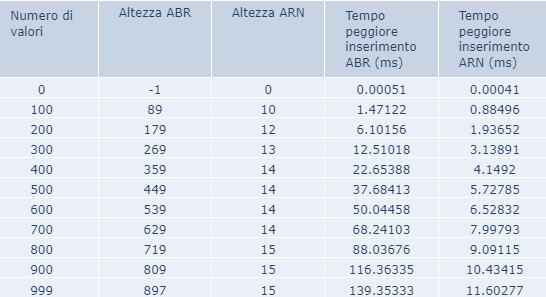
\includegraphics[]{TabellaPeggioreInserimento}
\caption{Tabella di ABR e ARN per Inserimento (caso peggiore)}
\label{fig:fig1}
\end{figure}
\\
\noindent \textit{\bf{Grafici a confronto:}} 
\begin{figure}[ht]
\centering
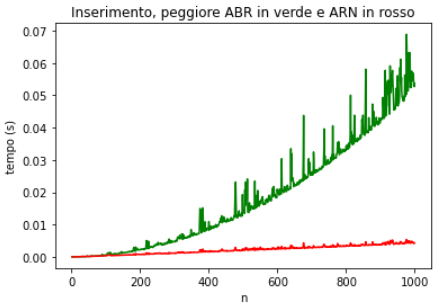
\includegraphics[width=.7\textwidth, height=.6\textheight, keepaspectratio]{GraficoInserimentoPeggiore}
\vspace{-5mm}
\caption{Grafici del tempo $t$ ($s$) di ABR e ARN per Inserimento (caso peggiore)}
\label{fig:fig2}
\end{figure}

\noindent \textit{\bf{Osservazioni:}} 

Il caso peggiore dell'inserimento, ottenuto inserendo nodi con chiavi in ordine crescente, mostra come questa operazione sia drammaticamente lenta all'aumentare dei nodi in un albero binario di ricerca sbilanciato, soprattutto se confrontata con la sua performance su un albero rosso-nero: il tempo massimo per un ABR, calcolato con 1000 nodi, è stato di $139 ms$, ovvero circa 10 volte maggiore rispetto ai $11 ms$ impiegati dall'ARN per lo stesso numero di elementi. \\
Notiamo inoltre che l'altezza dell'albero ARN è molto inferiore (15) rispetto all'altezza dell'albero ABR (897) . Come previsto, quindi, l'inserimento rischia di diventare un'operazione costosa per gli ABR: qualora sia probabile che l'ordine dei nodi da inserire sia quasi esclusivamente non (de)crescente, la scelta del tipo di albero da utilizzare deve obbligatoriamente favorire gli alberi rosso-neri. \\

% Caso peggiore di ricerca
\subsection {Caso peggiore di ricerca:} 
Si mostra di seguito il tempo di esecuzione nel caso peggiore, ottenuto inserendo nodi con chiavi in ordine crescente,  dei due algoritmi su un albero con numero di nodi crescenti da 1 a 1000. \\

\noindent \textit{\bf{Tabella a confronto:}} 
\begin{figure}[ht]
\centering
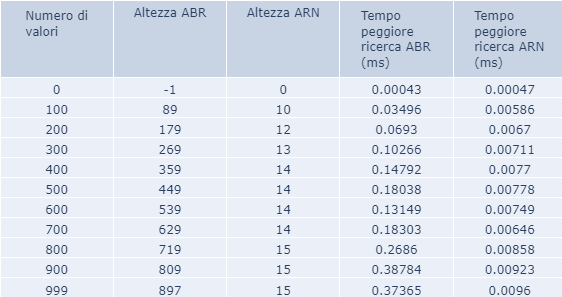
\includegraphics[]{TabellaPeggioreRicerca}
\caption{Tabella di ABR e ARN per Ricerca (caso peggiore)}
\label{fig:fig3}
\end{figure}
\\
\noindent \textit{\bf{Grafici a confronto:}}
\begin{figure}[ht]
\centering
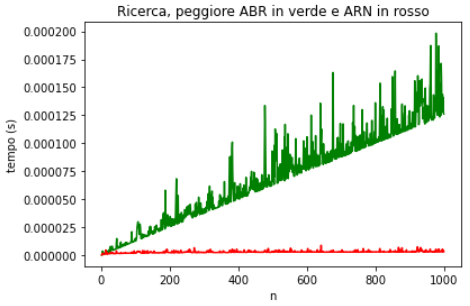
\includegraphics[width=.7\textwidth, height=.6\textheight, keepaspectratio]{GraficoRicercaPeggiore}
\vspace{-5mm}
\caption{Grafici del tempo $t$ ($s$) di ABR e ARN per Ricerca (caso peggiore)}
\label{fig:fig4}
\end{figure}

\noindent \textit{\bf{Osservazioni:}} 

La ricerca nel caso peggiore, eseguita per la chiave massima dell'albero (che si trova quindi nell'ultimo livello) costituisce il secondo caso in cui la scelta di un albero rosso-nero è palesemente migliore se i nodi vengono inseriti con un certo ordinamento. Pur essendo un'operazione veloce rispetto all'inserimento ($0.373 ms$ vs. i $139 ms$ per 1000 nodi dell'inserimento ABR), è comunque molto lenta se confrontata con la stessa operazione applicata su un ARN delle stesse dimensioni, che impiega $0,0096 ms$.\\


% Caso Random di inserimento
\subsection {Caso random di inserimento:} 
Si mostra di seguito il tempo di esecuzione nel caso medio (ottenuto inserendo nodi in ordine casuale) dei due algoritmi su un albero con numero di nodi crescenti da 1 a 1000. \\

\noindent \textit{\bf{Tabella a confronto:}}
\begin{figure}[ht]
\centering
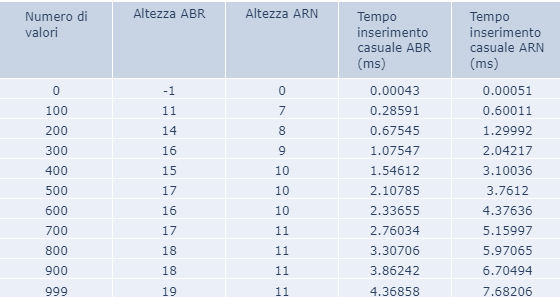
\includegraphics[]{TabellaInserimentoCasuale}
\caption{Tabella di ABR e ARN per Inserimento (caso random)}
\label{fig:fig5}
\end{figure}


\noindent \textit{\bf{Grafici a confronto:}}
\begin{figure}[ht]
\centering
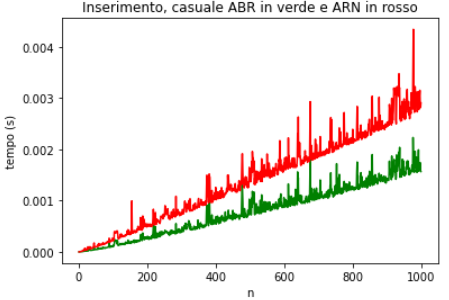
\includegraphics[width=.7\textwidth, height=.6\textheight, keepaspectratio]{GraficoInserimentoCasuale}
\vspace{-5mm}
\caption{Grafici del tempo $t$ ($s$) di ABR e ARN per Inserimento (caso random)}
\label{fig:fig6}
\end{figure}

\noindent \textit{\bf{Osservazioni:}}
Quanto visto nel caso peggiore non accade per il cosiddetto caso random, ovvero il caso medio degli alberi binari di ricerca: l'inserimento dei nodi in ordine casuale, come specificato nell'introduzione agli ABR, genera un albero approssimativamente bilanciato e quindi con tempi paragonabili a quelli degli ARN. Dai test sembrerebbe perfino che la scelta di un ABR sarebbe più conveniente rispetto a quella di un ARN, qualora si sappia a priori che i nodi non verranno aggiunti con un particolare ordinamento: un risultato probabilmente derivato dal fatto che un ARN, per essere bilanciato, ha bisogno di chiamare per ogni nodo la procedura \code{InsertFixup} che, pur avendo anch'essa tempo $O(lg(n))$, è comunque un insieme di operazioni aggiuntive che appesantiscono il programma.

% Caso Random di ricerca
\subsection {Caso random di ricerca:} 
Si mostra di seguito il tempo di esecuzione nel caso medio (ottenuto inserendo nodi in ordine casuale) dei due algoritmi su un albero con numero di nodi crescenti da 1 a 1000. \\

\noindent \textit{\bf{Tabella a confronto:}}
\begin{figure}[ht]
\centering
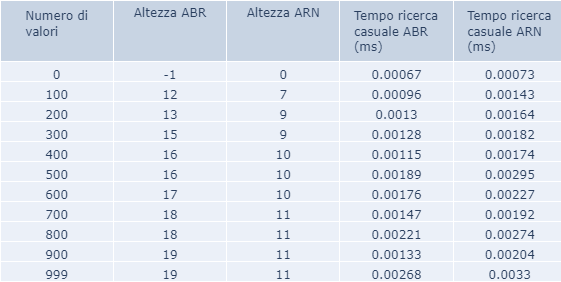
\includegraphics[]{TabellaRicercaCasuale}
\caption{Tabella di ABR e ARN per Ricerca (caso random)}
\label{fig:fig7}
\end{figure}


\noindent \textit{\bf{Grafici a confronto:}}
\begin{figure}[H]
\centering
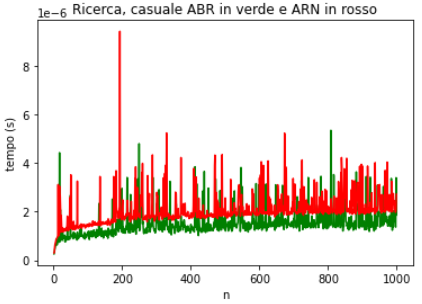
\includegraphics[width=.7\textwidth, height=.6\textheight, keepaspectratio]{GraficoRicercaCasuale}
\vspace{-5mm}
\caption{Grafici del tempo $t$ ($s$) di ABR e ARN per Ricerca (caso random)}
\label{fig:fig8}
\end{figure}

\noindent \textit{\bf{Osservazioni:}}

La ricerca nel caso random è invece circa equivalente alla ricerca nel caso peggiore di un ARN (riconfermando quindi il fatto che l'ARN non ha un caso peggiore perché è sempre bilanciato), ma questa volta anche per l'albero di ricerca binaria che, non avendo un solo nodo per ogni livello, ha un'altezza paragonabile a quella dell'albero rosso-nero.

% Caso attraversamento
\subsection {Attraversamento:} 
Si mostra di seguito il tempo di esecuzione nel caso medio (ottenuto inserendo nodi in ordine casuale) dei due algoritmi su un albero con numero di nodi crescenti da 1 a 1000. L'attraversamento è stato applicato nel caso in cui l'ordine di inserimento dei nodi fosse casuale. \\

\noindent \textit{\bf{Tabella a confronto:}} 
\begin{figure}[ht]
\centering
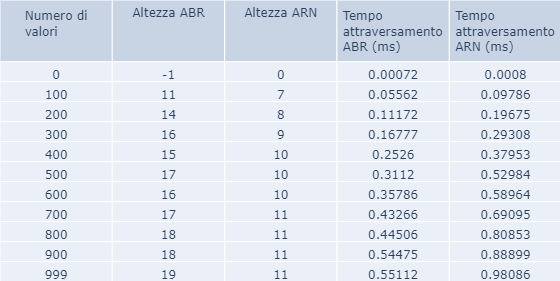
\includegraphics[]{TabellaAttraversamento}
\caption{Tabella di ABR e ARN per Attraversamento}
\label{fig:fig9}
\end{figure}


\noindent \textit{\bf{Grafici a confronto:}} 
\begin{figure}[ht]
\centering
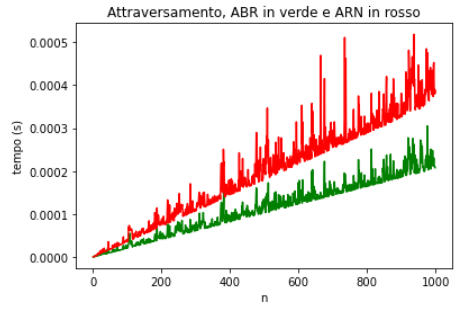
\includegraphics[width=.7\textwidth, height=.6\textheight, keepaspectratio]{GraficoAttraversamento}
\vspace{-5mm}
\caption{Grafici del tempo $t$ ($s$) di ABR e ARN per Attraversamento}
\label{fig:fig10}
\end{figure}

\noindent \textit{\bf{Osservazioni:}}

L'attraversamento inorder, che dovendo visitare tutti i nodi richiede $\Theta(n)$ a prescindere dall'altezza dell'albero, risulta come da aspettativa circa uguale sia per gli alberi binari di ricerca che per gli alberi rosso-neri ed è, a causa delle pochissime operazioni eseguite nel corpo della funzione, più veloce rispetto all'inserimento.


% Conclusioni
\section {Conclusioni}

Com'era intuibile, i risultati dei test ci portano a concludere che un albero rosso-nero è generalmente da preferire ad un semplice albero binario di ricerca, in quanto solitamente non si conosce l'ordine dei nodi che verranno  inseriti, e non è perciò possibile determinare a priori se nel tempo l'albero sarà bilanciato oppure no. Nel caso in cui ciò sia però noto, un ABR è equivalente ad un ARN, ed è anzi migliore nell'inserimento (data l'assenza della funzione ausiliaria \code{InsertFixup}). Anche se è stato analizzato un albero con al massimo 1000 nodi per il caso medio e peggiore, gli elementi utilizzati hanno permesso comunque di ottenere risultati sufficienti per le conclusioni cui si è giunti, dato che queste confermano le osservazioni teoriche fatte sugli alberi binari di ricerca e degli alberi rosso-neri.
In generale gli alberi rosso-neri risultano migliori in quanto, grazie alle loro proprietà, consentono all'albero di essere più bilanciato rispetto ad un albero binario di ricerca, qualsiasi siano i nodi da inserire.

\end{document}